% Options for packages loaded elsewhere
\PassOptionsToPackage{unicode}{hyperref}
\PassOptionsToPackage{hyphens}{url}
\PassOptionsToPackage{dvipsnames,svgnames,x11names}{xcolor}
%
\documentclass[
]{article}

\usepackage{amsmath,amssymb}
\usepackage{iftex}
\ifPDFTeX
  \usepackage[T1]{fontenc}
  \usepackage[utf8]{inputenc}
  \usepackage{textcomp} % provide euro and other symbols
\else % if luatex or xetex
  \usepackage{unicode-math}
  \defaultfontfeatures{Scale=MatchLowercase}
  \defaultfontfeatures[\rmfamily]{Ligatures=TeX,Scale=1}
\fi
\usepackage{lmodern}
\ifPDFTeX\else  
    % xetex/luatex font selection
\fi
% Use upquote if available, for straight quotes in verbatim environments
\IfFileExists{upquote.sty}{\usepackage{upquote}}{}
\IfFileExists{microtype.sty}{% use microtype if available
  \usepackage[]{microtype}
  \UseMicrotypeSet[protrusion]{basicmath} % disable protrusion for tt fonts
}{}
\makeatletter
\@ifundefined{KOMAClassName}{% if non-KOMA class
  \IfFileExists{parskip.sty}{%
    \usepackage{parskip}
  }{% else
    \setlength{\parindent}{0pt}
    \setlength{\parskip}{6pt plus 2pt minus 1pt}}
}{% if KOMA class
  \KOMAoptions{parskip=half}}
\makeatother
\usepackage{xcolor}
\setlength{\emergencystretch}{3em} % prevent overfull lines
\setcounter{secnumdepth}{5}
% Make \paragraph and \subparagraph free-standing
\makeatletter
\ifx\paragraph\undefined\else
  \let\oldparagraph\paragraph
  \renewcommand{\paragraph}{
    \@ifstar
      \xxxParagraphStar
      \xxxParagraphNoStar
  }
  \newcommand{\xxxParagraphStar}[1]{\oldparagraph*{#1}\mbox{}}
  \newcommand{\xxxParagraphNoStar}[1]{\oldparagraph{#1}\mbox{}}
\fi
\ifx\subparagraph\undefined\else
  \let\oldsubparagraph\subparagraph
  \renewcommand{\subparagraph}{
    \@ifstar
      \xxxSubParagraphStar
      \xxxSubParagraphNoStar
  }
  \newcommand{\xxxSubParagraphStar}[1]{\oldsubparagraph*{#1}\mbox{}}
  \newcommand{\xxxSubParagraphNoStar}[1]{\oldsubparagraph{#1}\mbox{}}
\fi
\makeatother

\usepackage{color}
\usepackage{fancyvrb}
\newcommand{\VerbBar}{|}
\newcommand{\VERB}{\Verb[commandchars=\\\{\}]}
\DefineVerbatimEnvironment{Highlighting}{Verbatim}{commandchars=\\\{\}}
% Add ',fontsize=\small' for more characters per line
\usepackage{framed}
\definecolor{shadecolor}{RGB}{241,243,245}
\newenvironment{Shaded}{\begin{snugshade}}{\end{snugshade}}
\newcommand{\AlertTok}[1]{\textcolor[rgb]{0.68,0.00,0.00}{#1}}
\newcommand{\AnnotationTok}[1]{\textcolor[rgb]{0.37,0.37,0.37}{#1}}
\newcommand{\AttributeTok}[1]{\textcolor[rgb]{0.40,0.45,0.13}{#1}}
\newcommand{\BaseNTok}[1]{\textcolor[rgb]{0.68,0.00,0.00}{#1}}
\newcommand{\BuiltInTok}[1]{\textcolor[rgb]{0.00,0.23,0.31}{#1}}
\newcommand{\CharTok}[1]{\textcolor[rgb]{0.13,0.47,0.30}{#1}}
\newcommand{\CommentTok}[1]{\textcolor[rgb]{0.37,0.37,0.37}{#1}}
\newcommand{\CommentVarTok}[1]{\textcolor[rgb]{0.37,0.37,0.37}{\textit{#1}}}
\newcommand{\ConstantTok}[1]{\textcolor[rgb]{0.56,0.35,0.01}{#1}}
\newcommand{\ControlFlowTok}[1]{\textcolor[rgb]{0.00,0.23,0.31}{\textbf{#1}}}
\newcommand{\DataTypeTok}[1]{\textcolor[rgb]{0.68,0.00,0.00}{#1}}
\newcommand{\DecValTok}[1]{\textcolor[rgb]{0.68,0.00,0.00}{#1}}
\newcommand{\DocumentationTok}[1]{\textcolor[rgb]{0.37,0.37,0.37}{\textit{#1}}}
\newcommand{\ErrorTok}[1]{\textcolor[rgb]{0.68,0.00,0.00}{#1}}
\newcommand{\ExtensionTok}[1]{\textcolor[rgb]{0.00,0.23,0.31}{#1}}
\newcommand{\FloatTok}[1]{\textcolor[rgb]{0.68,0.00,0.00}{#1}}
\newcommand{\FunctionTok}[1]{\textcolor[rgb]{0.28,0.35,0.67}{#1}}
\newcommand{\ImportTok}[1]{\textcolor[rgb]{0.00,0.46,0.62}{#1}}
\newcommand{\InformationTok}[1]{\textcolor[rgb]{0.37,0.37,0.37}{#1}}
\newcommand{\KeywordTok}[1]{\textcolor[rgb]{0.00,0.23,0.31}{\textbf{#1}}}
\newcommand{\NormalTok}[1]{\textcolor[rgb]{0.00,0.23,0.31}{#1}}
\newcommand{\OperatorTok}[1]{\textcolor[rgb]{0.37,0.37,0.37}{#1}}
\newcommand{\OtherTok}[1]{\textcolor[rgb]{0.00,0.23,0.31}{#1}}
\newcommand{\PreprocessorTok}[1]{\textcolor[rgb]{0.68,0.00,0.00}{#1}}
\newcommand{\RegionMarkerTok}[1]{\textcolor[rgb]{0.00,0.23,0.31}{#1}}
\newcommand{\SpecialCharTok}[1]{\textcolor[rgb]{0.37,0.37,0.37}{#1}}
\newcommand{\SpecialStringTok}[1]{\textcolor[rgb]{0.13,0.47,0.30}{#1}}
\newcommand{\StringTok}[1]{\textcolor[rgb]{0.13,0.47,0.30}{#1}}
\newcommand{\VariableTok}[1]{\textcolor[rgb]{0.07,0.07,0.07}{#1}}
\newcommand{\VerbatimStringTok}[1]{\textcolor[rgb]{0.13,0.47,0.30}{#1}}
\newcommand{\WarningTok}[1]{\textcolor[rgb]{0.37,0.37,0.37}{\textit{#1}}}

\providecommand{\tightlist}{%
  \setlength{\itemsep}{0pt}\setlength{\parskip}{0pt}}\usepackage{longtable,booktabs,array}
\usepackage{calc} % for calculating minipage widths
% Correct order of tables after \paragraph or \subparagraph
\usepackage{etoolbox}
\makeatletter
\patchcmd\longtable{\par}{\if@noskipsec\mbox{}\fi\par}{}{}
\makeatother
% Allow footnotes in longtable head/foot
\IfFileExists{footnotehyper.sty}{\usepackage{footnotehyper}}{\usepackage{footnote}}
\makesavenoteenv{longtable}
\usepackage{graphicx}
\makeatletter
\newsavebox\pandoc@box
\newcommand*\pandocbounded[1]{% scales image to fit in text height/width
  \sbox\pandoc@box{#1}%
  \Gscale@div\@tempa{\textheight}{\dimexpr\ht\pandoc@box+\dp\pandoc@box\relax}%
  \Gscale@div\@tempb{\linewidth}{\wd\pandoc@box}%
  \ifdim\@tempb\p@<\@tempa\p@\let\@tempa\@tempb\fi% select the smaller of both
  \ifdim\@tempa\p@<\p@\scalebox{\@tempa}{\usebox\pandoc@box}%
  \else\usebox{\pandoc@box}%
  \fi%
}
% Set default figure placement to htbp
\def\fps@figure{htbp}
\makeatother

\usepackage{booktabs}
\usepackage{longtable}
\usepackage{array}
\usepackage{multirow}
\usepackage{wrapfig}
\usepackage{float}
\usepackage{colortbl}
\usepackage{pdflscape}
\usepackage{tabu}
\usepackage{threeparttable}
\usepackage{threeparttablex}
\usepackage[normalem]{ulem}
\usepackage{makecell}
\usepackage{xcolor}
\makeatletter
\@ifpackageloaded{caption}{}{\usepackage{caption}}
\AtBeginDocument{%
\ifdefined\contentsname
  \renewcommand*\contentsname{Indholdsfortegnelse}
\else
  \newcommand\contentsname{Indholdsfortegnelse}
\fi
\ifdefined\listfigurename
  \renewcommand*\listfigurename{Figuroversigt}
\else
  \newcommand\listfigurename{Figuroversigt}
\fi
\ifdefined\listtablename
  \renewcommand*\listtablename{Tabeloversigt}
\else
  \newcommand\listtablename{Tabeloversigt}
\fi
\ifdefined\figurename
  \renewcommand*\figurename{Figur}
\else
  \newcommand\figurename{Figur}
\fi
\ifdefined\tablename
  \renewcommand*\tablename{Tabel}
\else
  \newcommand\tablename{Tabel}
\fi
}
\@ifpackageloaded{float}{}{\usepackage{float}}
\floatstyle{ruled}
\@ifundefined{c@chapter}{\newfloat{codelisting}{h}{lop}}{\newfloat{codelisting}{h}{lop}[chapter]}
\floatname{codelisting}{Liste}
\newcommand*\listoflistings{\listof{codelisting}{Listeoversigt}}
\makeatother
\makeatletter
\makeatother
\makeatletter
\@ifpackageloaded{caption}{}{\usepackage{caption}}
\@ifpackageloaded{subcaption}{}{\usepackage{subcaption}}
\makeatother

\ifLuaTeX
\usepackage[bidi=basic]{babel}
\else
\usepackage[bidi=default]{babel}
\fi
\babelprovide[main,import]{danish}
% get rid of language-specific shorthands (see #6817):
\let\LanguageShortHands\languageshorthands
\def\languageshorthands#1{}
\usepackage{bookmark}

\IfFileExists{xurl.sty}{\usepackage{xurl}}{} % add URL line breaks if available
\urlstyle{same} % disable monospaced font for URLs
\hypersetup{
  pdftitle={Arbejdsløshed - Ugeeksamen i Forecasting},
  pdfauthor={Christine Hegelund; Jing Wei; Marcus Nielsen},
  pdflang={da},
  colorlinks=true,
  linkcolor={blue},
  filecolor={Maroon},
  citecolor={Blue},
  urlcolor={Blue},
  pdfcreator={LaTeX via pandoc}}


\title{Arbejdsløshed - Ugeeksamen i Forecasting}
\author{Christine Hegelund \and Jing Wei \and Marcus Nielsen}
\date{2025-06-13}

\begin{document}
\maketitle


\maketitle
\thispagestyle{empty}
\begin{center}
\large{Forecasting Eksamen} \\[3em]
\end{center}
\begin{center}
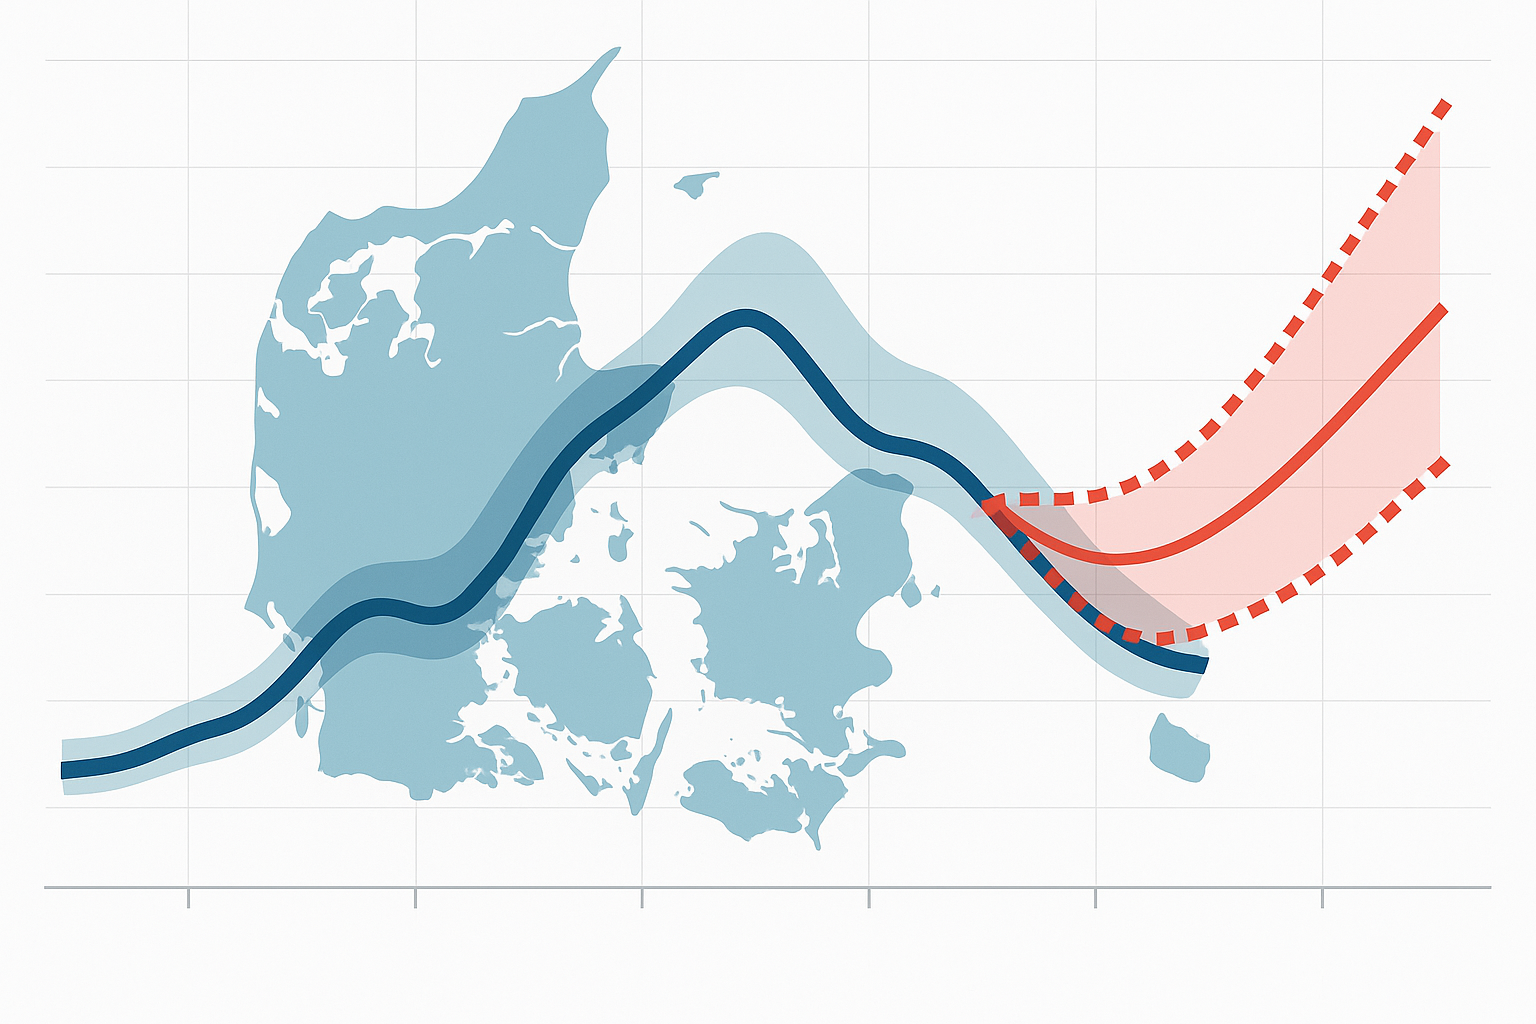
\includegraphics[width=0.9\textwidth]{fotos/forside.png} \\[2em]
\end{center}
\begin{center}
\fcolorbox{gray}{white}{
\parbox{0.8\textwidth}{
\centering
\textbf{Antal tegn (inkl. mellemrum): 97023}
}}
\end{center}
\begin{center}
\textbf{Vejledere:} \\
Bjarne Taulo Sørensen \\
\end{center}

\newpage

\addtocontents{toc}{\protect\setcounter{tocdepth}{-1}}

\section*{Tabel over figurer}\label{tabel-over-figurer}
\addcontentsline{toc}{section}{Tabel over figurer}

\thispagestyle{empty}

\newpage

\pagenumbering{arabic}
\setcounter{page}{1}
\tableofcontents
\newpage

\section{Introduktion}\label{introduktion}

Arbejdsløshedstal er en central indikator for et lands økonomiske
tilstand og udvikling. De påvirker både den enkelte borger og den
nationale økonomi og indgår som en væsentlig faktor i politiske og
økonomiske beslutningsprocesser. I takt med øget datatilgængelighed og
forbedrede statistiske værktøjer er det blevet muligt at analysere og
forudsige sådanne udviklingstræk med større præcision.

Denne opgave har til formål at modellere og forudsige udviklingen i
arbejdsløsheden i Danmark, fordelt på køn og region, med afsæt i
månedlige data for perioden januar 2007 til december 2019. Datasættet
består af ti tidsserier -- én for hver kombination af fem regioner og to
køn -- hvilket muliggør en detaljeret og differentieret analyse af både
strukturelle og sæsonbetingede mønstre i ledigheden.

Metodisk anvender analysen klassiske teknikker til tidsserieanalyse med
særligt fokus på modellerne ARIMA, ETS og en simpel benchmarkmodel
(Seasonal Naive). For hver serie estimeres de tre modeltyper, og deres
performance evalueres ved hjælp af forecast-metrikker som RMSE og MAPE.
Derudover inddrages elementer som STL-dekomposition, transformation af
data (log og Box-Cox), residualanalyse og test for hvid støj
(Ljung-Box).

Formålet er ikke blot at fremskrive arbejdsløsheden for året 2020, men
også at vurdere styrker og begrænsninger ved klassiske modeller til
tidsserieanalyse. Med dette udgangspunkt opstår spørgsmålet, hvordan
sådanne modeller bedst kan anvendes til at analysere og forudsige
arbejdsløsheden i Danmark, fordelt på region og køn.

\section{Problemformulering}\label{problemformulering}

Hvordan kan klassiske tidsseriemodeller anvendes til at analysere og
forudsige udviklingen i arbejdsløsheden i Danmark, fordelt på region og
køn?

For at besvare dette spørgsmål undersøges følgende delspørgsmål:

\begin{enumerate}
\def\labelenumi{\arabic{enumi}.}
\item
  Hvordan varierer arbejdsløshedens udvikling og sæsonmønstre på tværs
  af regioner og køn, og hvordan kan disse identificeres gennem
  eksplorativ dataanalyse og dekomposition?
\item
  Hvordan performer modellerne ARIMA, ETS og Seasonal Naive i forhold
  til hinanden, når det gælder præcision, residualstruktur og
  prognoseegenskaber?
\item
  Hvilke modeller er bedst egnede til at fremskrive
  arbejdsløshedstallene for 2020, og hvordan varierer resultater og
  usikkerhed på tværs af serierne?
\end{enumerate}

\subsection{Afgrænsning}\label{afgruxe6nsning}

Analysen er udelukkende baseret på de udleverede data og har fokus på
metodisk klarhed, reproducerbarhed og faglig konsistens. Eksterne
forklarende faktorer som COVID-19, konjunkturændringer og politiske
tiltag inddrages ikke.

Formålet er ikke at give strategiske eller forretningsmæssige
anbefalinger, men at demonstrere korrekt og velbegrundet anvendelse af
klassiske forecasting-metoder. Der lægges vægt på modellering,
evaluering og sammenligning af tidsseriemodeller i en struktureret
analytisk ramme.

\subsubsection{Anvendelse af
AI-værktøj}\label{anvendelse-af-ai-vuxe6rktuxf8j}

I udarbejdelsen af denne opgave er ChatGPT (GPT-4o) anvendt som et
støtteværktøj. Værktøjet har primært været anvendt til idéudvikling,
sproglig sparring, forbedring af formuleringers klarhed, grammatisk
gennemgang samt støtte ved udformning af enkelte kodestumper.
Anvendelsen har udelukkende omfattet sproglige, strukturelle og tekniske
elementer. Alt analytisk, fortolkende og konkluderende indhold er
selvstændigt udarbejdet af gruppens medlemmer.

\subsection{Definitioner/forkortelser}\label{definitionerforkortelser}

I dette afsnit afklares centrale begreber og forkortelser, der anvendes
gennem opgaven, for at sikre en ensartet forståelse.

\begin{itemize}
\tightlist
\item
  \textbf{ARIMA}: AutoRegressive Integrated Moving Average -- klassisk
  tidsseriemodel med trend og autokorrelation\\
\item
  \textbf{ETS}: Exponential Smoothing State Space Model --
  glatningsbaseret model til tidsserier med trend og sæson\\
\item
  \textbf{SNAÏVE}: Seasonal Naive -- benchmarkmodel, hvor forecast er
  lig med seneste sæsonværdi\\
\item
  \textbf{RMSE}: Root Mean Squared Error -- fejlmål hvor store
  afvigelser vægtes højt\\
\item
  \textbf{MAPE}: Mean Absolute Percentage Error -- fejl angivet i
  procent\\
\item
  \textbf{STL}: Seasonal-Trend decomposition using Loess -- metode til
  dekomponering af tidsserier\\
\item
  \textbf{CV}: Cross-validation -- validering af modeller via rullende
  trænings-/testvinduer\\
\item
  \textbf{Ljung-Box}: Test for autokorrelation i modelresidualer (white
  noise)
\end{itemize}

\subsection{Struktur}\label{struktur}

Opgaven er struktureret i overensstemmelse med en klassisk tilgang til
analyse af tidsserier og følger fire hovedfaser.

Først gennemføres en eksplorativ dataanalyse (EDA), hvor serierne
visualiseres og undersøges for tendenser og sæsonmønstre. Dette sker ved
hjælp af grafer, deskriptive statistikker og STL-dekomposition. Data
transformeres ved behov. Dernæst estimeres tre modeltyper for hver
serie: ARIMA, ETS og Seasonal Naive. Disse modeller valideres gennem
krydsvalidering og residualanalyse. På baggrund af modelperformance
foretages fremskrivninger af arbejdsløsheden for 2020 med tilhørende
prædiktionsintervaller. Afslutningsvis sammenlignes modellerne og
arbejdsløshedsniveauerne på tværs af regioner og køn, og der konkluderes
på analysens hovedspørgsmål.

\section{Data og forberedelse}\label{data-og-forberedelse}

Analysen er baseret på et datasæt med månedlige arbejdsløshedstal i
Danmark fra januar 2007 til december 2019. Data er opdelt på køn (mænd
og kvinder) og region (de fem danske regioner), hvilket resulterer i ti
separate tidsserier.

Datasættet er udleveret i forbehandlet format som en tsibble med korrekt
angivne indeks- og nøglevariabler.

\begin{Shaded}
\begin{Highlighting}[]
\CommentTok{\# Indlæs datasættet}
\NormalTok{data }\OtherTok{\textless{}{-}} \FunctionTok{read\_rds}\NormalTok{(}\StringTok{"data/Airidk\_long.rds"}\NormalTok{)}
\end{Highlighting}
\end{Shaded}

\section{Eksplorativ dataanalyse
(EDA)}\label{eksplorativ-dataanalyse-eda}

Dette afsnit har til formål at skabe et overblik over datasættets
struktur og variation forud for modelvalget. Gennem visualiseringer,
deskriptive statistikker og dekomponering undersøges arbejdsløshedens
udvikling på tværs af regioner og køn fra 2007 til 2019. Analysen
afdækker tendenser, sæsonmønstre og forskelle i niveau og variation.
STL-dekomposition anvendes til at isolere trend, sæson og residualer,
mens datatransformation vurderes for at sikre modellérbarhed.
Resultaterne danner det metodiske grundlag for den efterfølgende
modellering.

\subsection{Visualisering af udvikling og
mønstre}\label{visualisering-af-udvikling-og-muxf8nstre}

Formålet med dette afsnit er at identificere centrale mønstre og
karakteristika i arbejdsløshedsdataene -- herunder trends,
sæsonvariationer, regionale forskelle og forskelle mellem køn.
Visualiseringerne danner grundlag for valg af passende modeller til hver
tidsserie.

\subsubsection{Udvikling over tid}\label{udvikling-over-tid}

Dette afsnit har til formål at undersøge den overordnede udvikling i
arbejdsløsheden over tid -- opdelt på køn og region. Gennem
visualiseringer vurderes generelle trends og variationer i niveau, og
særlige hændelser som fx finanskrisen fremhæves.

\textbf{Figur 1: Udvikling i kvinders arbejdsløshed pr. region}

\begin{Shaded}
\begin{Highlighting}[]
\CommentTok{\# Figur 1}

\NormalTok{data }\SpecialCharTok{|\textgreater{}} 
  \FunctionTok{filter}\NormalTok{(kon }\SpecialCharTok{==} \StringTok{"Kvinder"}\NormalTok{) }\SpecialCharTok{|\textgreater{}} 
  \FunctionTok{autoplot}\NormalTok{(svalue) }\SpecialCharTok{+}
  \FunctionTok{labs}\NormalTok{(}
    \AttributeTok{title =} \StringTok{"Figur 1: Udvikling i kvinders arbejdsløshed pr. region"}\NormalTok{,}
    \AttributeTok{x =} \StringTok{"Tid"}\NormalTok{, }\AttributeTok{y =} \StringTok{"Arbejdsløse pr. 10.000 personer"}
\NormalTok{  ) }\SpecialCharTok{+}
  \FunctionTok{theme}\NormalTok{(}\AttributeTok{legend.title =} \FunctionTok{element\_blank}\NormalTok{())}
\end{Highlighting}
\end{Shaded}

\pandocbounded{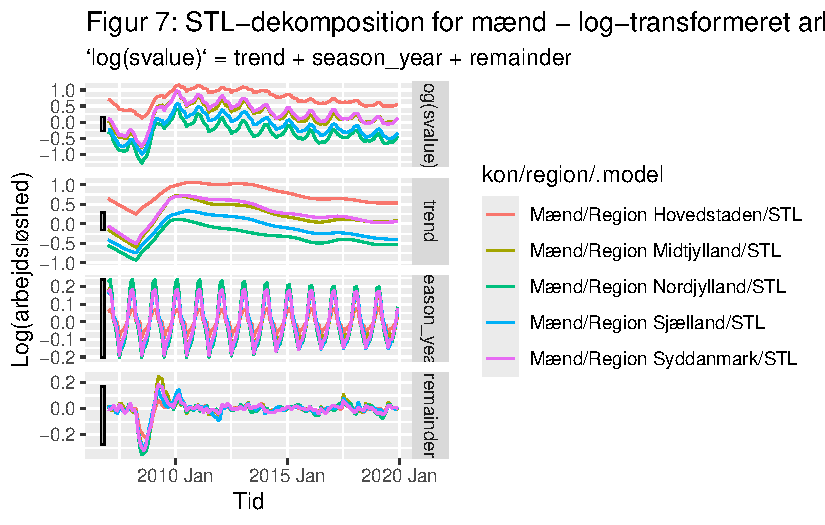
\includegraphics[keepaspectratio]{130625_Forecasting_files/figure-pdf/unnamed-chunk-2-1.pdf}}

Figuren viser den månedlige arbejdsløshed blandt kvinder i de fem danske
regioner fra 2007 til 2019. Der fremgår et tydeligt sæsonmønster med
højere ledighed i vintermånederne og lavere i sommerperioden. Niveauet
varierer regionalt, hvor Region Hovedstaden typisk ligger højest og
Nordjylland lavest. Samlet ses en faldende tendens efter finanskrisen.

\textbf{Figur 2: Udvikling i mænds arbejdsløshed pr. region}

\begin{Shaded}
\begin{Highlighting}[]
\CommentTok{\# Figur 2}

\NormalTok{data }\SpecialCharTok{|\textgreater{}} 
  \FunctionTok{filter}\NormalTok{(kon }\SpecialCharTok{==} \StringTok{"Mænd"}\NormalTok{) }\SpecialCharTok{|\textgreater{}} 
  \FunctionTok{autoplot}\NormalTok{(svalue) }\SpecialCharTok{+}
  \FunctionTok{labs}\NormalTok{(}
    \AttributeTok{title =} \StringTok{"Figur 2"}\NormalTok{,}
    \AttributeTok{subtitle =} \StringTok{"Udvikling i mænds arbejdsløshed pr. region"}\NormalTok{,}
    \AttributeTok{x =} \StringTok{"Tid"}\NormalTok{,}
    \AttributeTok{y =} \StringTok{"Arbejdsløse pr. 10.000 personer"}
\NormalTok{  ) }\SpecialCharTok{+}
  \FunctionTok{theme}\NormalTok{(}
    \AttributeTok{legend.title =} \FunctionTok{element\_blank}\NormalTok{()}
\NormalTok{  )}
\end{Highlighting}
\end{Shaded}

\pandocbounded{\includegraphics[keepaspectratio]{130625_Forecasting_files/figure-pdf/unnamed-chunk-3-1.pdf}}

Sammenlignet med kvinder ses større udsving og et generelt højere niveau
i mænds arbejdsløshed. Sæsonmønstrene er mere markante, og variationen
mellem regionerne er tydeligere -- især i Region Syddanmark og
Midtjylland, hvor krisen i 2008-2009 medfører et kraftigt midlertidigt
løft i ledigheden.

\textbf{Figur 3: Udvikling i arbejdsløshed hos mænd pr. region
(log-skala)}

\begin{Shaded}
\begin{Highlighting}[]
\CommentTok{\# Figur 3}

\NormalTok{data }\SpecialCharTok{|\textgreater{}} 
  \FunctionTok{filter}\NormalTok{(kon }\SpecialCharTok{==} \StringTok{"Mænd"}\NormalTok{) }\SpecialCharTok{|\textgreater{}} 
  \FunctionTok{autoplot}\NormalTok{(}\FunctionTok{log}\NormalTok{(svalue)) }\SpecialCharTok{+}
  \FunctionTok{labs}\NormalTok{(}
    \AttributeTok{title =} \StringTok{"Figur 3"}\NormalTok{,}
    \AttributeTok{subtitle =} \StringTok{"Udvikling i arbejdsløshed hos mænd pr. region (log{-}skala)"}\NormalTok{,}
    \AttributeTok{x =} \StringTok{"Tid"}\NormalTok{,}
    \AttributeTok{y =} \StringTok{"Log(arbejdsløse pr. 10.000 personer)"}
\NormalTok{  ) }\SpecialCharTok{+}
  \FunctionTok{theme\_minimal}\NormalTok{(}\AttributeTok{base\_size =} \DecValTok{12}\NormalTok{) }\SpecialCharTok{+}  \CommentTok{\# Giver et pænere layout}
  \FunctionTok{theme}\NormalTok{(}
    \AttributeTok{legend.title =} \FunctionTok{element\_blank}\NormalTok{(),        }\CommentTok{\# Fjerner titel fra farvelegenden}
    \AttributeTok{plot.title =} \FunctionTok{element\_text}\NormalTok{(}\AttributeTok{face =} \StringTok{"bold"}\NormalTok{)  }\CommentTok{\# Fremhæver titlen lidt}
\NormalTok{  )}
\end{Highlighting}
\end{Shaded}

\pandocbounded{\includegraphics[keepaspectratio]{130625_Forecasting_files/figure-pdf/unnamed-chunk-4-1.pdf}}

Da mændenes tidsserier generelt udviser højere niveauer og større
variation end kvindernes, undersøges i figur 3, om en log-transformation
kan give et mere stabilt og jævnt udgangspunkt for modellering. Formålet
er ikke at sammenligne direkte med det oprindelige plot, men at vurdere,
om transformationen reducerer skævhed og fremhæver relative ændringer på
en måde, der kan være fordelagtig for videre analyse.

Ud over de langsigtede trends spiller sæsonvariation en vigtig rolle for
arbejdsløsheden. Det undersøges nærmere i de følgende visualiseringer.

\subsubsection{Sæsonmønstre}\label{suxe6sonmuxf8nstre}

For bedre at forstå de tilbagevendende variationer i arbejdsløsheden
undersøges sæsonmønstre separat for mænd og kvinder. Der anvendes både
sæsonplots og subserieplots, som fremhæver gentagne mønstre over måneder
og år.

\textbf{Figur 4: Sæsonmønster for mænd pr. region}

\begin{Shaded}
\begin{Highlighting}[]
\CommentTok{\#Figur 4: Sæsonmønster for mænd pr. region}

\NormalTok{data }\SpecialCharTok{|\textgreater{}} 
  \FunctionTok{filter}\NormalTok{(kon }\SpecialCharTok{==} \StringTok{"Mænd"}\NormalTok{) }\SpecialCharTok{|\textgreater{}} 
  \FunctionTok{gg\_season}\NormalTok{(svalue) }\SpecialCharTok{+}
  \FunctionTok{labs}\NormalTok{(}
    \AttributeTok{title =} \StringTok{"Figur 4"}\NormalTok{,}
    \AttributeTok{subtitle =} \StringTok{"Sæsonvariation i arbejdsløshed pr. region"}\NormalTok{,}
    \AttributeTok{x =} \StringTok{"Måned"}\NormalTok{,}
    \AttributeTok{y =} \StringTok{"Arbejdsløshed"}
\NormalTok{  )}
\end{Highlighting}
\end{Shaded}

\pandocbounded{\includegraphics[keepaspectratio]{130625_Forecasting_files/figure-pdf/unnamed-chunk-5-1.pdf}}

Figur 4 viser sæsonmønstre i mænds arbejdsløshed fordelt på regioner.
Hver farvet linje repræsenterer et år, og linjernes forløb illustrerer,
hvordan arbejdsløsheden typisk er højest i årets begyndelse
(januar--marts) og lavest i sommermånederne (juni--august). Mønsteret er
relativt konsistent på tværs af år og regioner, hvilket understøtter
tilstedeværelsen af en stabil sæsonkomponent i mænds ledighed. De
højeste niveauer ses i Region Hovedstaden, mens Region Sjælland og
Region Nordjylland ligger lavere. Bemærk især det markante fald fra
marts til juni, som gentager sig på tværs af årstal.

\textbf{Figur 5: Sæsonmønster for kvinder pr. region}

\begin{Shaded}
\begin{Highlighting}[]
\CommentTok{\#Figur 5: Sæsonmønster for kvinder pr. region}

\NormalTok{data }\SpecialCharTok{|\textgreater{}} 
  \FunctionTok{filter}\NormalTok{(kon }\SpecialCharTok{==} \StringTok{"Kvinder"}\NormalTok{) }\SpecialCharTok{|\textgreater{}} 
  \FunctionTok{gg\_season}\NormalTok{(svalue) }\SpecialCharTok{+}
  \FunctionTok{labs}\NormalTok{(}
    \AttributeTok{title =} \StringTok{"Figur 5"}\NormalTok{,}
    \AttributeTok{subtitle =} \StringTok{"Sæsonvariation i arbejdsløshed pr. region"}\NormalTok{,}
    \AttributeTok{x =} \StringTok{"Måned"}\NormalTok{,}
    \AttributeTok{y =} \StringTok{"Arbejdsløshed"}
\NormalTok{  )}
\end{Highlighting}
\end{Shaded}

\pandocbounded{\includegraphics[keepaspectratio]{130625_Forecasting_files/figure-pdf/unnamed-chunk-6-1.pdf}}

Sammenlignet med mænd er sæsonudsvingene blandt kvinder mindre udtalte,
og udviklingen fremstår mere jævn og stabil på tværs af årene.
Niveauforskellene mellem regionerne er bevaret, men udsvingene over
måneder er mere afdæmpede. Det indikerer en lavere volatilitet i
kvinders arbejdsløshed og en mere ensartet sæsonprofil.

\textbf{Figur 6: Subserieplot for mænd pr. måned og region}

\begin{Shaded}
\begin{Highlighting}[]
\CommentTok{\#Figur 6}

\NormalTok{data }\SpecialCharTok{|\textgreater{}} 
  \FunctionTok{filter}\NormalTok{(kon }\SpecialCharTok{==} \StringTok{"Mænd"}\NormalTok{) }\SpecialCharTok{|\textgreater{}} 
  \FunctionTok{gg\_subseries}\NormalTok{(svalue) }\SpecialCharTok{+}
  \FunctionTok{labs}\NormalTok{(}
    \AttributeTok{title =} \StringTok{"Figur 6"}\NormalTok{,}
    \AttributeTok{subtitle =} \StringTok{"Subserieplot for mænd pr. måned og region"}\NormalTok{,}
    \AttributeTok{x =} \StringTok{"Måned"}\NormalTok{,}
    \AttributeTok{y =} \StringTok{"Arbejdsløshed"}
\NormalTok{  )}
\end{Highlighting}
\end{Shaded}

\pandocbounded{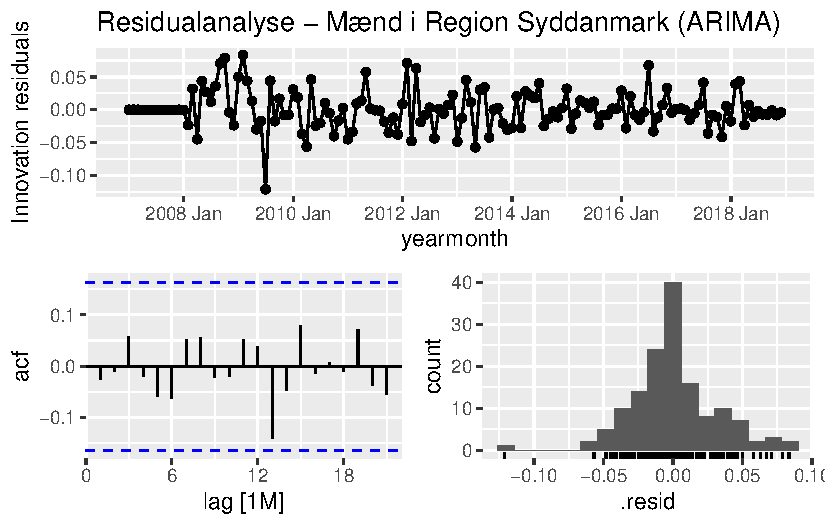
\includegraphics[keepaspectratio]{130625_Forecasting_files/figure-pdf/unnamed-chunk-7-1.pdf}}

Figur 6 viser udviklingen i mænds arbejdsløshed fordelt på måneder og
regioner, hvor hver facetteret celle repræsenterer en måned. Den sorte
linje viser udviklingen over tid, mens den blå streg repræsenterer
gennemsnittet. Det ses, at arbejdsløsheden konsekvent topper i årets
første måneder og falder hen over sommeren. Desuden er udsvingene mellem
år særligt store i vinterhalvåret, hvilket understreger en høj
sæsonafhængighed og volatilitet i mænds ledighedsniveau. Mønstret er
gennemgående i alle regioner, om end niveauet varierer.

\textbf{Figur 7: Subserieplot for kvinder pr. måned og region}

\begin{Shaded}
\begin{Highlighting}[]
\CommentTok{\#Figur 7}
\NormalTok{data }\SpecialCharTok{|\textgreater{}} 
  \FunctionTok{filter}\NormalTok{(kon }\SpecialCharTok{==} \StringTok{"Kvinder"}\NormalTok{) }\SpecialCharTok{|\textgreater{}} 
  \FunctionTok{gg\_subseries}\NormalTok{(svalue) }\SpecialCharTok{+}
  \FunctionTok{labs}\NormalTok{(}
    \AttributeTok{title =} \StringTok{"Figur 7"}\NormalTok{,}
    \AttributeTok{subtitle =} \StringTok{"Subserieplot for kvinder pr. måned og region"}\NormalTok{,}
    \AttributeTok{x =} \StringTok{"Måned"}\NormalTok{,}
    \AttributeTok{y =} \StringTok{"Arbejdsløshed"}
\NormalTok{  )}
\end{Highlighting}
\end{Shaded}

\pandocbounded{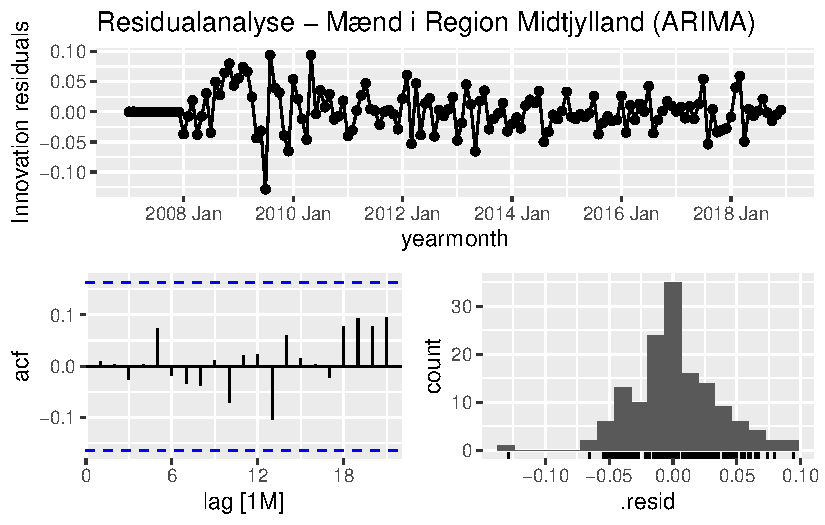
\includegraphics[keepaspectratio]{130625_Forecasting_files/figure-pdf/unnamed-chunk-8-1.pdf}}

Sammenlignet med mænd viser kvinder tilsvarende sæsonmønstre med højere
ledighed i årets begyndelse og lavere i sommermånederne. Udsvingene er
dog mindre markante, og variationen mellem år er mindre tydelig.
Mønstret fremstår mere stabilt og jævnt fordelt på tværs af regioner,
hvilket tyder på lavere volatilitet i kvindernes arbejdsløshed.

Udover sæsonmæssige udsving varierer arbejdsløsheden betydeligt på tværs
af både geografi og køn. Dette undersøges nærmere i de følgende
visualiseringer.

\subsubsection{Regionale og kønsmæssige
forskelle}\label{regionale-og-kuxf8nsmuxe6ssige-forskelle}

I dette afsnit rettes fokus mod samspillet mellem køn og region. Der
undersøges, hvordan forskelle i arbejdsløshedsniveau og -mønstre
varierer både mellem regioner og mellem mænd og kvinder.
Visualiseringerne præsenteres i forskellige facetteringer for at
fremhæve de vigtigste forskelle.

\textbf{Figur 8: Arbejdsløshed fordelt på regioner -- opdelt efter køn}

\begin{Shaded}
\begin{Highlighting}[]
\CommentTok{\#"Figur 8: Arbejdsløshed fordelt på regioner – opdelt efter køn"}

\NormalTok{data }\SpecialCharTok{|\textgreater{}} 
  \FunctionTok{autoplot}\NormalTok{(svalue) }\SpecialCharTok{+}
  \FunctionTok{aes}\NormalTok{(}\AttributeTok{colour =}\NormalTok{ region) }\SpecialCharTok{+}
  \FunctionTok{facet\_wrap}\NormalTok{(}\SpecialCharTok{\textasciitilde{}}\NormalTok{ kon) }\SpecialCharTok{+}
  \FunctionTok{labs}\NormalTok{(}
    \AttributeTok{title =} \StringTok{"Figur 8"}\NormalTok{,}
    \AttributeTok{subtitle =} \StringTok{"Arbejdsløshed fordelt på regioner – opdelt efter køn"}\NormalTok{,}
    \AttributeTok{y =} \StringTok{"Arbejdsløse pr. 10.000 personer"}\NormalTok{, }\AttributeTok{x =} \StringTok{"Tid"}
\NormalTok{  ) }\SpecialCharTok{+}
  \FunctionTok{theme}\NormalTok{(}\AttributeTok{legend.position =} \StringTok{"bottom"}\NormalTok{, }\AttributeTok{legend.title =} \FunctionTok{element\_blank}\NormalTok{())}
\end{Highlighting}
\end{Shaded}

\pandocbounded{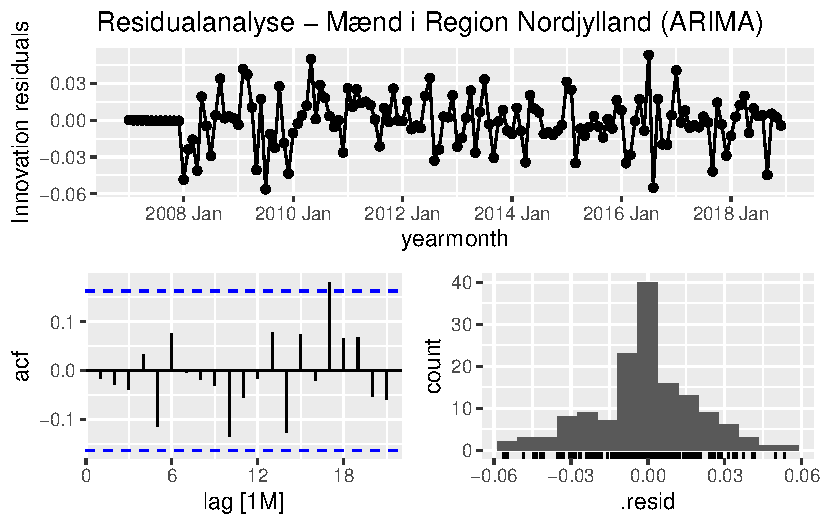
\includegraphics[keepaspectratio]{130625_Forecasting_files/figure-pdf/unnamed-chunk-9-1.pdf}}

Figur 8 viser udviklingen i arbejdsløsheden for mænd og kvinder i
separate paneler, hvor farverne angiver de fem danske regioner. Denne
visning gør det muligt at sammenligne geografiske forskelle inden for
hvert køn. Region Hovedstaden har konsekvent det højeste
ledighedsniveau, mens Nordjylland ligger lavest. Blandt mænd ses både
højere niveauer og større udsving, særligt under og efter finanskrisen.
Kvindernes udvikling er generelt mere stabil og glidende. Bemærk, at
forskellene mellem regionerne fremstår tydeligere blandt kvinder,
hvilket kan tyde på mere vedvarende strukturelle forskelle.

\textbf{Figur 9: Arbejdsløshed fordelt på køn -- opdelt efter region}

\begin{Shaded}
\begin{Highlighting}[]
\CommentTok{\# Figur 9: Arbejdsløshed fordelt på køn – opdelt efter region}

\NormalTok{data }\SpecialCharTok{|\textgreater{}} 
  \FunctionTok{autoplot}\NormalTok{(svalue) }\SpecialCharTok{+}
  \FunctionTok{aes}\NormalTok{(}\AttributeTok{colour =}\NormalTok{ kon, }\AttributeTok{group =}\NormalTok{ kon) }\SpecialCharTok{+}
  \FunctionTok{facet\_wrap}\NormalTok{(}\SpecialCharTok{\textasciitilde{}}\NormalTok{ region, }\AttributeTok{scales =} \StringTok{"free\_y"}\NormalTok{) }\SpecialCharTok{+}
  \FunctionTok{labs}\NormalTok{(}
    \AttributeTok{title =} \StringTok{"Figur 9"}\NormalTok{,}
    \AttributeTok{subtitle =} \StringTok{"Arbejdsløshed fordelt på køn – opdelt efter region"}\NormalTok{,}
    \AttributeTok{y =} \StringTok{"Arbejdsløse pr. 10.000 personer"}\NormalTok{, }\AttributeTok{x =} \StringTok{"Tid"}\NormalTok{,}
    \AttributeTok{colour =} \StringTok{"Køn"}
\NormalTok{  ) }\SpecialCharTok{+}
  \FunctionTok{scale\_colour\_manual}\NormalTok{(}
    \AttributeTok{values =} \FunctionTok{c}\NormalTok{(}\StringTok{"Mænd"} \OtherTok{=} \StringTok{"steelblue"}\NormalTok{, }\StringTok{"Kvinder"} \OtherTok{=} \StringTok{"hotpink"}\NormalTok{)}
\NormalTok{  ) }\SpecialCharTok{+}
  \FunctionTok{theme}\NormalTok{(}\AttributeTok{legend.position =} \StringTok{"bottom"}\NormalTok{, }\AttributeTok{legend.title =} \FunctionTok{element\_blank}\NormalTok{())}
\end{Highlighting}
\end{Shaded}

\pandocbounded{\includegraphics[keepaspectratio]{130625_Forecasting_files/figure-pdf/unnamed-chunk-10-1.pdf}}

Hvor Figur 8 fokuserede på at sammenligne regioner inden for hvert køn,
giver Figur 9 et omvendt perspektiv: her sammenlignes køn i hver af de
fem danske regioner. Mænd har generelt højere ledighed og mere markante
udsving end kvinder -- særligt i perioden omkring finanskrisen.
Forskellene mellem kønnene er relativt ensartede på tværs af regioner,
men mønstret bekræfter, at mænds ledighed både topper højere og varierer
mere over tid. Kvinders ledighed er lavere og følger en mere stabil
udvikling. Figuren understøtter dermed beslutningen om at analysere
serierne individuelt.

Samlet set viser figurerne, at arbejdsløsheden varierer tydeligt mellem
regioner og køn. Denne variation understøtter behovet for at behandle
hver tidsserie separat i den videre analyse. Som næste skridt anvendes
deskriptive statistikker til at opsummere centrale forskelle i niveau og
udsving mellem serierne.

\subsection{Deskriptive statistikker}\label{deskriptive-statistikker}

For at supplere graferne anvendes deskriptive statistikker som
gennemsnit, spredning, minimum og maksimum. De opsummerer niveau og
variation i arbejdsløsheden pr. region og køn (Hyndman \&
Athanasopoulos, 2021). Statistikkerne giver et hurtigt overblik over
forskelle mellem grupper og hjælper med at identificere serier med høj
volatilitet. Det bidrager til at vurdere, hvor der kan være behov for
særlig opmærksomhed i den videre modellering.

\begin{Shaded}
\begin{Highlighting}[]
\CommentTok{\# Beregning}
\NormalTok{deskriptiv }\OtherTok{\textless{}{-}}\NormalTok{ data }\SpecialCharTok{|\textgreater{}} 
  \FunctionTok{as\_tibble}\NormalTok{() }\SpecialCharTok{|\textgreater{}}
  \FunctionTok{group\_by}\NormalTok{(region, kon) }\SpecialCharTok{|\textgreater{}} 
  \FunctionTok{summarise}\NormalTok{(}
    \AttributeTok{Gennemsnit =} \FunctionTok{mean}\NormalTok{(svalue, }\AttributeTok{na.rm =} \ConstantTok{TRUE}\NormalTok{),}
    \StringTok{\textasciigrave{}}\AttributeTok{Standardafvigelse}\StringTok{\textasciigrave{}} \OtherTok{=} \FunctionTok{sd}\NormalTok{(svalue, }\AttributeTok{na.rm =} \ConstantTok{TRUE}\NormalTok{),}
    \AttributeTok{Minimum =} \FunctionTok{min}\NormalTok{(svalue, }\AttributeTok{na.rm =} \ConstantTok{TRUE}\NormalTok{),}
    \AttributeTok{Maksimum =} \FunctionTok{max}\NormalTok{(svalue, }\AttributeTok{na.rm =} \ConstantTok{TRUE}\NormalTok{),}
    \AttributeTok{.groups =} \StringTok{"drop"}
\NormalTok{  )}

\CommentTok{\# Visning}
\NormalTok{deskriptiv }\SpecialCharTok{|\textgreater{}} 
  \FunctionTok{kable}\NormalTok{(}\AttributeTok{format =} \StringTok{"markdown"}\NormalTok{, }\AttributeTok{digits =} \DecValTok{2}\NormalTok{, }\AttributeTok{caption =} \StringTok{"Tabel 1: Deskriptiv statistik per region og køn"}\NormalTok{) }\SpecialCharTok{|\textgreater{}} 
  \FunctionTok{kable\_styling}\NormalTok{(}\AttributeTok{full\_width =} \ConstantTok{FALSE}\NormalTok{, }\AttributeTok{position =} \StringTok{"center"}\NormalTok{, }\AttributeTok{bootstrap\_options =} \FunctionTok{c}\NormalTok{(}\StringTok{"striped"}\NormalTok{, }\StringTok{"hover"}\NormalTok{)) }\SpecialCharTok{|\textgreater{}} 
  \FunctionTok{row\_spec}\NormalTok{(}\DecValTok{0}\NormalTok{, }\AttributeTok{bold =} \ConstantTok{TRUE}\NormalTok{, }\AttributeTok{background =} \StringTok{"\#f0f0f0"}\NormalTok{)}
\end{Highlighting}
\end{Shaded}

\begin{longtable}[t]{llrrrr}
\caption{Tabel 1: Deskriptiv statistik per region og køn}\\
\toprule
\cellcolor[HTML]{f0f0f0}{\textbf{region}} & \cellcolor[HTML]{f0f0f0}{\textbf{kon}} & \cellcolor[HTML]{f0f0f0}{\textbf{Gennemsnit}} & \cellcolor[HTML]{f0f0f0}{\textbf{Standardafvigelse}} & \cellcolor[HTML]{f0f0f0}{\textbf{Minimum}} & \cellcolor[HTML]{f0f0f0}{\textbf{Maksimum}}\\
\midrule
Region Hovedstaden & Kvinder & 2.07 & 0.36 & 1.13 & 2.67\\
Region Hovedstaden & Mænd & 2.17 & 0.52 & 1.13 & 3.18\\
Region Midtjylland & Kvinder & 1.27 & 0.25 & 0.58 & 1.72\\
Region Midtjylland & Mænd & 1.29 & 0.44 & 0.45 & 2.62\\
Region Nordjylland & Kvinder & 0.67 & 0.10 & 0.38 & 1.09\\
\addlinespace
Region Nordjylland & Mænd & 0.74 & 0.23 & 0.28 & 1.50\\
Region Sjælland & Kvinder & 0.86 & 0.17 & 0.45 & 1.20\\
Region Sjælland & Mænd & 0.92 & 0.30 & 0.37 & 1.78\\
Region Syddanmark & Kvinder & 1.24 & 0.26 & 0.60 & 1.76\\
Region Syddanmark & Mænd & 1.37 & 0.47 & 0.47 & 2.65\\
\bottomrule
\end{longtable}

Tabel 1 opsummerer arbejdsløsheden på tværs af regioner og køn.
Gennemsnittet viser det generelle niveau, mens standardafvigelsen giver
et mål for variation over tid. Mænd har generelt højere gennemsnit og
større udsving end kvinder, særligt i Region Hovedstaden og Syddanmark.
Omvendt ses lavere og mere stabile niveauer i Nordjylland, især blandt
kvinder. Minimums- og maksimumværdier understøtter indtrykket af høj
volatilitet i visse serier -- hvilket kan få betydning for modelvalget i
næste fase.

\subsection{STL-dekomposition}\label{stl-dekomposition}

For at opnå en bedre forståelse af de strukturelle komponenter i
arbejdsløshedsserierne anvendes STL-dekomposition (Seasonal-Trend
decomposition using Loess). Metoden adskiller tidsserier i tre
komponenter: trend, sæson og remainder (Hyndman \& Athanasopoulos,
2021). Det giver indblik i, hvor meget af variationen der kan forklares
af langsigtede bevægelser, gentagne sæsonmønstre eller kortsigtede,
uregelmæssige udsving.

Da særligt mændenes serier udviser høje niveauer og større variation, er
alle serier log-transformeret forud for dekompositionen. Denne
transformation stabiliserer variansen og gør det lettere at sammenligne
komponenterne på tværs af regioner og køn.

STL anvendes her på de log-transformerede serier for henholdsvis kvinder
og mænd i hver region. Resultaterne præsenteres i figur 10 og 11.

\begin{Shaded}
\begin{Highlighting}[]
\NormalTok{kvinder\_STL }\OtherTok{\textless{}{-}}\NormalTok{ data }\SpecialCharTok{|\textgreater{}} 
  \FunctionTok{filter}\NormalTok{(kon }\SpecialCharTok{==} \StringTok{"Kvinder"}\NormalTok{) }\SpecialCharTok{|\textgreater{}} 
  \FunctionTok{model}\NormalTok{(}\AttributeTok{STL =} \FunctionTok{STL}\NormalTok{(}\FunctionTok{log}\NormalTok{(svalue), }\AttributeTok{robust =} \ConstantTok{TRUE}\NormalTok{))}

\NormalTok{kvinder\_STL }\SpecialCharTok{|\textgreater{}} 
  \FunctionTok{components}\NormalTok{() }\SpecialCharTok{|\textgreater{}} 
  \FunctionTok{autoplot}\NormalTok{() }\SpecialCharTok{+}
  \FunctionTok{labs}\NormalTok{(}
    \AttributeTok{title =} \StringTok{"Figur 10: STL{-}dekomposition for kvinder"}\NormalTok{,}
    \AttributeTok{subtitle =} \StringTok{"Log{-}transformeret arbejdsløshed pr. region"}\NormalTok{,}
    \AttributeTok{x =} \StringTok{"Tid"}\NormalTok{,}
    \AttributeTok{y =} \StringTok{"Log(arbejdsløshed)"}
\NormalTok{  )}
\end{Highlighting}
\end{Shaded}

\pandocbounded{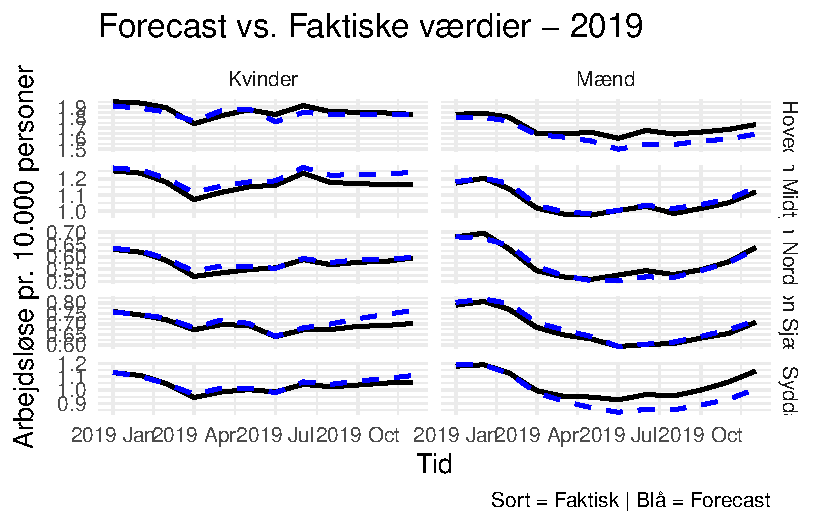
\includegraphics[keepaspectratio]{130625_Forecasting_files/figure-pdf/unnamed-chunk-11-1.pdf}}

\textbf{Figur 10: STL-dekomposition for kvinder -- log-transformeret
arbejdsløshed pr. region} Figur 10 viser STL-dekompositionen for kvinder
i de fem danske regioner. Der ses tydelige sæsonmønstre med
tilbagevendende lavpunkter i sommermånederne og højere ledighed i
vinterhalvåret. Trends varierer mellem regionerne: Region Hovedstaden
udviser generelt højere ledighed, mens Nordjylland og Sjælland ligger
lavere. Residualerne ligger stabilt omkring nul, hvilket indikerer, at
modellen formår at fange de dominerende strukturer i data.

\begin{Shaded}
\begin{Highlighting}[]
\NormalTok{mænd\_STL }\OtherTok{\textless{}{-}}\NormalTok{ data }\SpecialCharTok{|\textgreater{}} 
  \FunctionTok{filter}\NormalTok{(kon }\SpecialCharTok{==} \StringTok{"Mænd"}\NormalTok{) }\SpecialCharTok{|\textgreater{}}
  \FunctionTok{model}\NormalTok{(}\AttributeTok{STL =} \FunctionTok{STL}\NormalTok{(}\FunctionTok{log}\NormalTok{(svalue), }\AttributeTok{robust =} \ConstantTok{TRUE}\NormalTok{))}

\NormalTok{mænd\_STL }\SpecialCharTok{|\textgreater{}} 
  \FunctionTok{components}\NormalTok{() }\SpecialCharTok{|\textgreater{}} 
  \FunctionTok{autoplot}\NormalTok{() }\SpecialCharTok{+}
  \FunctionTok{labs}\NormalTok{(}
    \AttributeTok{title =} \StringTok{"Figur 11: STL{-}dekomposition for mænd"}\NormalTok{,}
    \AttributeTok{subtitle =} \StringTok{"Log{-}transformeret arbejdsløshed pr. region"}\NormalTok{,}
    \AttributeTok{x =} \StringTok{"Tid"}\NormalTok{,}
    \AttributeTok{y =} \StringTok{"Log(arbejdsløshed)"}
\NormalTok{  )}
\end{Highlighting}
\end{Shaded}

\pandocbounded{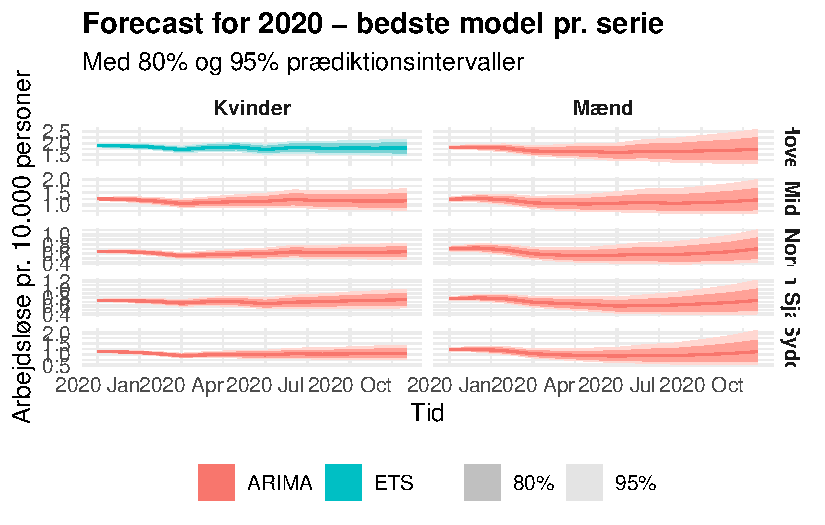
\includegraphics[keepaspectratio]{130625_Forecasting_files/figure-pdf/unnamed-chunk-12-1.pdf}}

\textbf{Figur 11: STL-dekomposition for mænd -- log-transformeret
arbejdsløshed pr. region} Figur 11 viser tilsvarende dekomposition for
mænd. Her ses en tilsvarende stærk sæsonkomponent, men med mere markante
udsving og højere ledighedsniveauer -- især efter finanskrisen. Trends
følger samme overordnede forløb som for kvinder, men afvigelserne er
større. Dette bekræfter tidligere observationer om højere volatilitet i
mænds ledighed. Residualkomponenten er mere varierende, hvilket kan
indikere, at nogle udsving ikke fanges fuldt ud af modellen.

Disse observationer fra STL-dekompositionen bekræfter, at både trend og
sæsonmønstre varierer betydeligt på tværs af serierne. Det understreger
behovet for modeller, der kan tilpasses hver series struktur, hvilket
vil blive præsenteret i det følgende afsnit.

\section{Modelvalg}\label{modelvalg}

I dette afsnit estimeres og sammenlignes tre klassiske modeltyper,
ARIMA, ETS og benchmarkmodellen SNaive, for hver tidsserie (region ×
køn). Hver modeltype har forskellige antagelser og fordele og kan fange
forskellige karakteristika i data, såsom trend, sæson og
autokorrelation. Modelvalget foretages automatisk for hver serie via
fable-pakken, og resultaterne anvendes i den efterfølgende validering og
forecast.

\subsection{Valgte modeltyper}\label{valgte-modeltyper}

\textbf{ARIMA (AutoRegressive Integrated Moving Average)}\\
ARIMA-modeller anvendes til at modellere tidsserier med autokorrelation
og ikke-stationaritet. De kombinerer autoregressive (AR) led, differens
(I) for at opnå stationaritet, og glidende gennemsnit (MA) led til at
modellere fejl. Ved at inkludere sæsonkomponenter (SARIMA) kan modellen
håndtere årligt gentagende mønstre. ARIMA er særligt velegnet til serier
med langsigtede trends og strukturelle skift, hvor tidligere værdier har
stor indflydelse på den nuværende tilstand (jf. Hyndman \&
Athanasopoulos, kap. 9).

\textbf{ETS (Exponential Smoothing State Space Model)}\\
ETS-modeller benytter eksponentiel glatning til at vægte nyere
observationer højere og beskriver tidsserier ud fra tre elementer: fejl,
trend og sæson. Hver komponent kan være additiv eller multiplicativ
afhængigt af dataens karakter. ETS egner sig godt til serier med
tydelige strukturer og sæsonrytmer, især når der ikke er behov for at
modellere autokorrelation direkte (jf. kap. 8).

\textbf{SNAÏVE (Seasonal Naive)}\\
SNaive er en enkel benchmarkmodel, der baserer hvert forecast på den
tilsvarende værdi fra samme sæson i den foregående periode. Modellen
fanger sæsonmønstre, men tager ikke højde for trend eller afhængighed i
data. Den anvendes til at vurdere, om mere komplekse modeller giver en
mærkbart bedre forecast-præcision (jf. kap. 3 og 8).

\subsection{Modellering i praksis}\label{modellering-i-praksis}

Ved hjælp af fable-pakken estimeres de tre modeller automatisk for hver
af de ti tidsserier på baggrund af data fra 2007 til 2019. Herefter
genereres forecasts for 2020 med tilhørende prædiktionsintervaller.
Prognoserne visualiseres, så man kan sammenligne modellernes adfærd på
tværs af regioner og køn.

\begin{Shaded}
\begin{Highlighting}[]
\CommentTok{\# Estimér modeller for hele perioden 2007–2019}
\NormalTok{models }\OtherTok{\textless{}{-}}\NormalTok{ data }\SpecialCharTok{|\textgreater{}} 
  \FunctionTok{model}\NormalTok{(}
    \AttributeTok{ARIMA  =} \FunctionTok{ARIMA}\NormalTok{(svalue),}
    \AttributeTok{ETS    =} \FunctionTok{ETS}\NormalTok{(svalue),}
    \AttributeTok{SNaive =} \FunctionTok{SNAIVE}\NormalTok{(svalue)}
\NormalTok{  )}

\CommentTok{\# Udtræk modelinformation med glance()}
\CommentTok{\# Brug TIDY til at få modelstruktur}
\NormalTok{modelinfo }\OtherTok{\textless{}{-}}\NormalTok{ models }\SpecialCharTok{|\textgreater{}}
  \FunctionTok{glance}\NormalTok{() }\SpecialCharTok{|\textgreater{}}
  \FunctionTok{select}\NormalTok{(kon, region, .model, AICc)}


\CommentTok{\# Vis tabellen}
\NormalTok{modelinfo }\SpecialCharTok{|\textgreater{}} 
  \FunctionTok{arrange}\NormalTok{(kon, region) }\SpecialCharTok{|\textgreater{}} 
  \FunctionTok{kable}\NormalTok{(}\AttributeTok{format =} \StringTok{"markdown"}\NormalTok{,}
        \AttributeTok{caption =} \StringTok{"Tabel 2: Automatisk valgte modelstrukturer for hver serie (region × køn)"}\NormalTok{,}
        \AttributeTok{align =} \StringTok{"l"}\NormalTok{) }\SpecialCharTok{|\textgreater{}} 
  \FunctionTok{kable\_styling}\NormalTok{(}\AttributeTok{full\_width =} \ConstantTok{FALSE}\NormalTok{, }\AttributeTok{position =} \StringTok{"center"}\NormalTok{, }\AttributeTok{bootstrap\_options =} \FunctionTok{c}\NormalTok{(}\StringTok{"striped"}\NormalTok{, }\StringTok{"hover"}\NormalTok{)) }\SpecialCharTok{|\textgreater{}} 
  \FunctionTok{row\_spec}\NormalTok{(}\DecValTok{0}\NormalTok{, }\AttributeTok{bold =} \ConstantTok{TRUE}\NormalTok{, }\AttributeTok{background =} \StringTok{"\#f0f0f0"}\NormalTok{)}
\end{Highlighting}
\end{Shaded}

\begin{longtable}[t]{llll}
\caption{Tabel 2: Automatisk valgte modelstrukturer for hver serie (region × køn)}\\
\toprule
\cellcolor[HTML]{f0f0f0}{\textbf{kon}} & \cellcolor[HTML]{f0f0f0}{\textbf{region}} & \cellcolor[HTML]{f0f0f0}{\textbf{.model}} & \cellcolor[HTML]{f0f0f0}{\textbf{AICc}}\\
\midrule
Kvinder & Region Hovedstaden & ARIMA & -519.59277\\
Kvinder & Region Hovedstaden & ETS & -106.04957\\
Kvinder & Region Hovedstaden & SNaive & NA\\
Kvinder & Region Midtjylland & ARIMA & -559.62392\\
Kvinder & Region Midtjylland & ETS & -186.73947\\
\addlinespace
Kvinder & Region Midtjylland & SNaive & NA\\
Kvinder & Region Nordjylland & ARIMA & -794.48456\\
Kvinder & Region Nordjylland & ETS & -420.44010\\
Kvinder & Region Nordjylland & SNaive & NA\\
Kvinder & Region Sjælland & ARIMA & -714.46022\\
\addlinespace
Kvinder & Region Sjælland & ETS & -355.53652\\
Kvinder & Region Sjælland & SNaive & NA\\
Kvinder & Region Syddanmark & ARIMA & -615.90506\\
Kvinder & Region Syddanmark & ETS & -194.25088\\
Kvinder & Region Syddanmark & SNaive & NA\\
\addlinespace
Mænd & Region Hovedstaden & ARIMA & -451.76084\\
Mænd & Region Hovedstaden & ETS & -94.42293\\
Mænd & Region Hovedstaden & SNaive & NA\\
Mænd & Region Midtjylland & ARIMA & -365.22171\\
Mænd & Region Midtjylland & ETS & 24.67626\\
\addlinespace
Mænd & Region Midtjylland & SNaive & NA\\
Mænd & Region Nordjylland & ARIMA & -536.74821\\
Mænd & Region Nordjylland & ETS & -202.87509\\
Mænd & Region Nordjylland & SNaive & NA\\
Mænd & Region Sjælland & ARIMA & -524.52351\\
\addlinespace
Mænd & Region Sjælland & ETS & -271.66140\\
Mænd & Region Sjælland & SNaive & NA\\
Mænd & Region Syddanmark & ARIMA & -387.29279\\
Mænd & Region Syddanmark & ETS & -55.07382\\
Mænd & Region Syddanmark & SNaive & NA\\
\bottomrule
\end{longtable}

Tabel 2 viser de modelstrukturer og AICc-værdier, som fable automatisk
har estimeret for hver tidsserie. Modelvalg inden for ARIMA og ETS sker
med udgangspunkt i AICc, som balancerer modeltilpasning og kompleksitet
og forebygger overfitting, særligt ved kortere tidsserier.
ARIMA-modellerne inkluderer ofte sæsonled og har i flere tilfælde høje
AR- eller MA-ordener, hvilket peger på både sæsonvariation og
autokorrelation i data. ETS-modellerne spænder over forskellige
kombinationer af additive og multiplicative komponenter afhængigt af
serien.

SNaive-modellen er medtaget som benchmark og har ingen tilhørende
AICc-værdier, da den ikke bygger på en statistisk
sandsynlighedsstruktur. Den anvendes i stedet som reference i den
efterfølgende forecast-validering.

At modelvalgene varierer på tværs af regioner og køn bekræfter behovet
for en individualiseret tilgang og underbygger den differentierede
modelstrategi, der anvendes i analysen.

\begin{Shaded}
\begin{Highlighting}[]
\CommentTok{\# Forecast for 12 måneder frem}
\NormalTok{fc }\OtherTok{\textless{}{-}}\NormalTok{ models }\SpecialCharTok{|\textgreater{}} \FunctionTok{forecast}\NormalTok{(}\AttributeTok{h =} \StringTok{"12 months"}\NormalTok{)}

\CommentTok{\# Plot forecasts pr. serie}
\NormalTok{fc }\SpecialCharTok{|\textgreater{}} 
  \FunctionTok{autoplot}\NormalTok{(data) }\SpecialCharTok{+}
  \FunctionTok{labs}\NormalTok{(}
    \AttributeTok{title =} \StringTok{"Figur 12"}\NormalTok{,}
    \AttributeTok{subtitle =} \StringTok{"Forecasts for 2020 – pr. region og køn"}\NormalTok{,}
    \AttributeTok{y =} \StringTok{"Arbejdsløse pr. 10.000 personer"}\NormalTok{,}
    \AttributeTok{x =} \StringTok{"Tid"}
\NormalTok{  ) }\SpecialCharTok{+}
  \FunctionTok{facet\_wrap}\NormalTok{(}\SpecialCharTok{\textasciitilde{}}\NormalTok{ kon }\SpecialCharTok{+}\NormalTok{ region, }\AttributeTok{scales =} \StringTok{"free\_y"}\NormalTok{) }\SpecialCharTok{+}
  \FunctionTok{theme\_minimal}\NormalTok{()}
\end{Highlighting}
\end{Shaded}

\pandocbounded{\includegraphics[keepaspectratio]{130625_Forecasting_files/figure-pdf/unnamed-chunk-13-1.pdf}}

Figur 12 viser forecasts og historiske data for hver kombination af
region og køn. Visualiseringen giver et overblik over, hvordan de tre
modeller tilpasser sig de forskellige seriers niveau og variation. Dette
danner udgangspunkt for den efterfølgende vurdering af modellernes
præcision.

\section{Modelvalidering}\label{modelvalidering}

\subsection{Time series
cross-validation}\label{time-series-cross-validation}

\subsection{Evaluering med RMSE og
MAPE}\label{evaluering-med-rmse-og-mape}

\subsection{Valg af bedste model pr.
serie}\label{valg-af-bedste-model-pr.-serie}

\subsection{Test for hvid støj}\label{test-for-hvid-stuxf8j}

\section{Forecasting}\label{forecasting}

\subsection{Træning og forecast for
2020}\label{truxe6ning-og-forecast-for-2020}

\subsection{Prædiktionsintervaller}\label{pruxe6diktionsintervaller}

\subsection{Visualisering af
forecasts}\label{visualisering-af-forecasts}

\subsection{Centrale prognoseværdier}\label{centrale-prognosevuxe6rdier}

\section{Sammenligning og
fortolkning}\label{sammenligning-og-fortolkning}

\subsection{Sammenligning på tværs af
serier}\label{sammenligning-puxe5-tvuxe6rs-af-serier}

\subsection{Tendenser mellem regioner og
køn}\label{tendenser-mellem-regioner-og-kuxf8n}

\section{Konklusion}\label{konklusion}

\newpage

\section{Kildeliste}\label{kildeliste}

Hyndman, R. J., \& Athanasopoulos, G. (2021).~\emph{Forecasting:
principles and practice}~(3rd ed.). OTexts.~https://otexts.com/fpp3/

\newpage

\section{Bilagsoversigt}\label{bilagsoversigt}

\begin{itemize}
\tightlist
\item
  Bilag 1: Udleverede Powerpointpræsentationer v. Michael Freundlich:
  Chefkonsulent, Erhvervsservice og facility
\end{itemize}




\end{document}
